\documentclass{article}


% Use the postscript times font!

% --- Packages ---
\usepackage{times}
\usepackage{rldmsubmit}
\usepackage{enumerate, amsmath, hyperref, amsthm,gensymb, subfig, verbatim, amssymb, dashrule, tikz, bbm, booktabs, bm}
\usepackage[framemethod=TikZ]{mdframed}
\usepackage[numbers]{natbib}

\newcommand{\dnote}[1]{\textcolor{blue}{Dave: #1}}
\newcommand{\enote}[1]{\textcolor{purple}{Emily: #1}}
\newcommand{\mc}{\mathcal}
\newcommand\ddfrac[2]{\frac{\displaystyle #1}{\displaystyle #2}}
\DeclareMathOperator*{\argmax}{argmax}

% --- Misc. ---
\hbadness=10000 % No "underfull hbox" messages.

% --- Meta Info ---
\title{Improving Solar Panel Efficiency Using Reinforcement Learning}

% Authors
\author{
David Abel, Emily Reif, Michael L. Littman \\
Department of Computer Science\\
Brown University \\
Providence, RI 02912 \\
\texttt{david\_abel@brown.edu, emily\_reif@brown.edu, mlittman@cs.brown.edu} \\
}


% --- Begin Document ---
\begin{document}
\maketitle


% -----------------
% -- Abstract --
% -----------------
\begin{abstract}
Solar panels sustainably harvest energy from the sun. To improve performance, panels are often equipped with a tracking mechanism that computes the sun's position in the sky throughout the day. Based on the tracker's estimate of the sun's location, a controller orients the panel to minimize the angle of incidence between solar radiant energy and the photovoltaic cells on the surface of the panel, increasing total energy harvested. Prior work has developed efficient tracking algorithms that accurately compute the sun's location to facilitate solar tracking and control.
%
However, always pointing a panel directly at the sun does not account for diffuse irradiance in the sky, reflected irradiance from the ground and surrounding surfaces, or changing weather conditions (such as cloud coverage), all of which are contributing factors to the total energy harvested by a solar panel.
%
In this work, we show that a reinforcement-learning (RL) approach can increase the total energy harvested by solar panels by learning to dynamically account for such other factors. We advocate for the use of RL for solar panel control due to its {\it effectiveness}, {\it negligible cost}, and {\it versatility}. Our contribution is twofold: (1) an adaption of typical RL algorithms to the task of improving solar panel performance, and (2) an experimental validation in simulation based on typical solar and irradiance models for experimenting with solar panel control.
%
We evaluate the utility of various RL approaches compared to an idealized controller, an efficient state-of-the-art direct tracking algorithm, and a fixed panel in our simulated environment. We experiment across different time scales, in different places on earth, and with dramatically different percepts (sun coordinates and raw images of the sky with and without clouds), consistently demonstrating that simple RL algorithms improve over existing baselines.
\end{abstract}


\keywords{
Solar panels, Renewable Energy, Computational Sustainability
}

% ----------------------
% -- Introduction --
% ----------------------
\newpage
\section{Introduction}
% Solare Panels and Solar Tracking.
Solar energy offers a pollution free and sustainable means of harvesting energy directly from the sun. Considerable effort has been directed toward maximizing the efficiency of end-to-end solar systems, including the design of photovoltaic cells~\cite{Jervase2001,li2012molecular}, engineering new photovoltaic architectures and materials~\cite{li2005high}, and solar tracking systems~\cite{camacho2012control}. Solar tracking is especially important for maximizing performance of solar panels~\cite{Eke2012,Rizk2008,King2001}. Given the proper sensors and hardware, a tracking algorithm can compute the relative location of the sun in the sky throughout the day, and a controller can orient the panel to point at the sun, illustrated in Figure~\ref{fig:solar}. Its goal is to minimize the angle of incidence between incoming solar radiant energy and the grid of photovoltaic cells, as in~\citet{Eke2012,Benghanem2011,King2001} and~\citet{kalogirou1996design}.

Prior work has consistently demonstrated that panels using a tracking system increase the total energy by a substantial amount:~\citet{Eke2012} report that a dual-axis tracker yielded 71 kW/h, compared to a fixed panel's yield of 52 kW/h on the same day. They also report energy harvesting gains of dual-axis tracking systems over fixed systems varying from 15\% to 40\%, depending on the time of year.~\citet{mousazadeh2009review} report that gains from tracking can vary between 0\% and 100\%, while~\citet{clifford2004design} report a gain of $23\%$ due to tracking in simulation. Solar tracking and control result in non-trivial benefits in solar photovoltaic systems.

% Diagram with labels
\begin{figure}[b!]
%\begin{center}
\subfloat{\includegraphics[scale=0.355]{figures/relevant_quantities.png}}
\subfloat{\begin{tabular}{lcc}
\toprule
Quantity& Variable& Range \\
\midrule
latitude& $L$& $[-\pi, \pi]$ \\
longitude& $G$&  $\left[-\frac{\pi}{2}, \frac{\pi}{2}\right]$\\
%declination& $\delta$ & $\left[-\frac{\pi}{2}, \frac{\pi}{2}\right]$ \\
%hour angle& $H$& $\left[-\frac{\pi}{2}, \frac{\pi}{2}\right]$ \\
%zenith& $z$& $[0,\pi]$ \\
azimuth& $\Gamma$& $[-\pi, \pi]$ \\
altitude& $\alpha$& $[-\pi, \pi]$ \\
panel NS angle& $\nu$& $[-\pi, \pi]$ \\
panel EW angle& $\omega$& $[-\pi, \pi]$ \\
ground reflective index& $\rho$& $[0,1]$ \\
\bottomrule
\end{tabular}}
%\caption{In the solar panel control problem, the panel changes its orientation over time to maximize total exposure to solar radiant energy.}
\label{fig:solar}
%\end{center}
\end{figure}

% Previous algorithms
Recent work in solar tracking has focused on algorithms that are sufficiently accurate to inform control of panels, building on the early work of~\citet{spencer1971fourier,walraven1978calculating} and~\citet{michalsky1988astronomical}. The algorithm introduced by~\citet{reda2004solar} computes the sun's location in the sky within $\pm 0.0003\degree$ of accuracy, achieving the highest degree of accuracy of any known algorithm, but is computationally inefficient to the point of impracticality.~\citet{Grena2008} overcomes these inefficiencies with a tracking algorithm that requires an order of magnitude fewer calculations while still achieving $0.0027\degree$ of accuracy.

% Limitations
However, prior literature suggests that a variety of factors contribute to the performance of a panel~\cite{King2001}, and thus, pointing a panel directly at the sun is not always optimal behavior. Specifically, the total solar irradiance falling on a panel is a combination of {\it direct}, {\it reflective}, and {\it diffuse} irradiance~\cite{Benghanem2011}. The diffuse irradiance typically varies between $15\%$ and $55\%$ of direct irradiance depending on factors like cloud coverage and the time of day~\cite{peterson1981ratio}, while a case study by the Cold Climate Housing Research Center in Fairbanks, Alaska reports reflective irradiance varying from $5\%$ to $25\%$ of direct irradiance~\cite{colgan2010}. The reflective irradiance varies heavily based on the percentage of irradiance reflected off the surrounding ground surface: Typical values for this percentage given by~\citet{mcevoy2003practical} vary between $17\%$ (soil), $25\%$ (grass), $55\%$ (concrete), and $90\%$ (snow). Additionally, changing weather and atmospheric conditions can affect the optimal panel orientation~\cite{Kelly2009}. Thus, optimal performance may involve prioritizing reflective or diffuse irradiance when direct sunlight is not available.

% Others require extra hardware.
There are two additional shortcomings to the classical tracking approach. First, tracking algorithms take as input a variety of data that require additional hardware such as a barometer, thermometer, or GPS~\cite{Grena2012}, increasing the total cost and system complexity. Second, tracking algorithms are only accurate for a fixed window of time: The algorithm of~\citet{Grena2008} is noted as accurate until 2023 AD (due to the subtle movements of the earth and sun), while the algorithms in~\citet{Grena2012} are reported as accurate until 2110 AD.

% RL for solar tracking.
In this work, we advocate for the use of RL to optimize solar panel performance. In this setting, a learned solar panel controller can account for weather change, cloud coverage, and diverse reflective indices of surroundings, offering an efficient yet adaptive solution that can optimize for the given availability of each type of solar irradiance without the need for complex hardware, regardless of the location or year. Our primary contribution is twofold:
\begin{enumerate}
\item The advancement of a highly relevant problem as an application area for RL, including a high fidelity simulation built using recently introduced models of solar irradiance.
\item The validation of the utility of RL approaches for solar panel control.
\end{enumerate}

% ----------------------
% -- Background --
% ----------------------
\section{Background}

We begin with some background on solar tracking.

% Solar Tracking Background
\subsection{Solar Tracking}
The amount of solar radiant energy contacting a surface on the earth's surface (per unit area, per unit time) is called {\it irradiance}~\cite{goswami2000principles}.  We denote the total irradiance hitting a panel as $R_t$, which, per the models developed by~\citet{kamali2006estimating}, is approximated by the sum of the {\it direct} irradiance, $R_d$, {\it diffuse} irradiance (light from the sky), $R_f$, and {\it reflective} irradiance, $R_r$ (reflected off the ground or other surfaces). Each of these components is modified by a scalar, $\theta_d, \theta_f, \theta_r \in [0,1]$, denoting the effect of the angle of incidence between oncoming solar rays and the panel's orientation, yielding the total:
\begin{equation}
R_t = R_d \theta_d + R_f \theta_f + R_r \theta_r
\label{eq:total_rads}
\end{equation}
Additionally, the components $R_d$ and $R_f$ are known to be effected by cloud coverage~\cite{li2004overcast,pfister2003cloud,tzoumanikas2016effect}. We attend to these details in describing our simulation in Section~\ref{sec:simulation}.

% Controller for solar panel.
A controller for a solar panel then seeks to maximize total irradiance, $R_t$, hitting the panel's surface. In the case of solar trackers, a running assumption is that it is near optimal to orient the panel such that its normal vector is pointing at the sun, and thus arises the necessity for accurate solar tracking algorithms. There are many types of tracking methods, only a few of which we discuss in this work; for an in depth survey of solar tracking techniques, see~\citet{mousazadeh2009review}.

% --- Table of Quantities ---
{\renewcommand{\arraystretch}{1.2}%
\begin{figure}
\centering
\begin{tabular}{lcc}
\toprule
Quantity& Variable& Range \\
\midrule
latitude& $L$& $[-\pi, \pi]$ \\
longitude& $G$&  $\left[-\frac{\pi}{2}, \frac{\pi}{2}\right]$\\
%declination& $\delta$ & $\left[-\frac{\pi}{2}, \frac{\pi}{2}\right]$ \\
%hour angle& $H$& $\left[-\frac{\pi}{2}, \frac{\pi}{2}\right]$ \\
%zenith& $z$& $[0,\pi]$ \\
azimuth& $\Gamma$& $[-\pi, \pi]$ \\
altitude& $\alpha$& $[-\pi, \pi]$ \\
panel NS angle& $\nu$& $[-\pi, \pi]$ \\
panel EW angle& $\omega$& $[-\pi, \pi]$ \\
ground reflective index& $\rho$& $[0,1]$ \\
\bottomrule
\end{tabular}
\caption{Relevant solar tracking and irradiance variables.}
\end{figure}

% Agents
%\subsubsection{RL Agents}
%
%We experiment with two relatively simple learning agents: $Q$-Learning and SARSA, each with a linear function approximator to estimate $Q^*$. To test the significance of modeling the sequential aspects of the problem, we also conduct experiments with $Q$-Learning with $\gamma=0$ (so it only maximizes immediate return) and LinUCB~\cite{li2010contextual}, a standard approach to non-sequential Contextual Bandits. We chose each of the linear approximators to illustrate that online, efficient, and lightweight algorithms can be effective in the domain. We chose not to experiment with any Deep RL agents~\cite{mnih2015human}, as Deep RL typically requires more computational power (and often GPUs), which may be unavailable or limited in the real solar panel setting. However, this could be an area of further exploration. We now turn to describing the details of our simulation.

% ----------------------
% --- Simulation ---
% ----------------------
\section{Simulation}
\label{sec:simulation}

We introduce a high fidelity simulated environment to validate the use of RL for solar panel control. There are four basic stages to the simulation:
\begin{enumerate}
\item Computing the sun's location in the sky, relative to the panel.
\item Computing $R_d, R_f$, and $R_r$.
\item Computing $\theta_d, \theta_f$, and $\theta_r$.
\item Generating percepts.
\end{enumerate}

% (Step 1) Sun location in the sky.
\subsection{Sun's location in the sky}
For a given latitude, longitude, year, month, day, and time, we simulate the relative positions of the sun to the specified location on earth. Our simulation computes the sun's altitude $\alpha$ (angle: degrees above the horizon) and azimuth $\Gamma$ (angle: clockwise degrees along the horizon relative to North) using the highly accurate tracker algorithm from~\citet{reda2004solar} implemented in the open source library \texttt{pysolar}.\footnote{\url{pysolar.org}} Due to space constraints, we do not express the full computation. Note, however, that a quicker approximation (also available in \texttt{pysolar}) is given by:
% --- Math about \alpha and \Gamma ---
\begin{align}
\alpha = \arcsin(\cos L \cos \delta \cos H + \sin L \sin \delta), \hspace{4mm} \Gamma = \arcsin\left(\frac{\cos \delta \sin H}{\cos \alpha}\right).
\end{align}
For the full details, see~\citet{reda2004solar}.

% (Step 2) Irradiance.
\subsection{Computing $\pmb{R_d, R_f, R_r}$}
Given the sun's altitude $\alpha$ and azimuth $\Gamma$, we compute the $R_d, R_f,$ and $R_d$ from the models of~\citet{threlkeld1957direct,Liu1960} and~\citet{masters2013renewable}.\footnote{Higher fidelity models are known to exist, such as those developed by~\citet{andersen1980comments,klein1977calculation} and~\citet{kamali2006estimating}. In particular, our estimates of the diffuse and reflective radiation are simple relative to the best known models. (This choice was made to make the simulation more efficient.)}
% --- Math about R_d, R_f, R_r ---
\begin{align}
R_d = A e^{-km}, \hspace{2mm} R_f = C \cdot R_d, \hspace{2mm} R_r = \rho R_d (\sin \alpha + C),
\end{align}
where $A$ is the apparent extraterrestrial flux, $k$ is the optical depth, $m$ is the air mass ratio, $\rho \in [0,1)$ is a reflective index (albedo) denoting how reflective the ground is, and $C$ is a sky diffusion factor, each given by the approximations:
\begin{align}
m&=\frac{1}{\sin \alpha}, \hspace{2mm} A = 1160 + \sin \left(0.99 n- 271\right), \hspace{2mm} k =0.174 + 0.035 \sin\left( 0.99 n - 99\right), \hspace{2mm} C=0.095 + 0.04 \sin\left(0.99 n-99\right),
\end{align}
where $n \in [1:365]$ is a day of the year.

% (Step 3) angles.
\subsection{Computing $\pmb{\theta_d, \theta_f, \theta_r}$}
Given the two angles describing the panel's orientation ($\nu$: north-south tilt, $\omega$: east-west tilt), we simulate the amount of total irradiance actually hitting the panel's surface. The models of~\citet{masters2013renewable} compute $\theta_t$ in terms of the $\cos$-similarity between the panel's normal vector, $\vec{p}$, and the sun's vector, $\vec{s}$, (with the panel as the origin):
% --- Math about \theta_d, \theta_f, \theta_r. ---
\begin{align*}
\vec{p} &= \begin{bmatrix} \sin(\nu)  \cos(\omega)& \cos(\nu)  \cos(\omega)& \cos(\nu) \cos(\omega) \end{bmatrix}, \\
\vec{s} &= \begin{bmatrix} \sin(\pi - \Gamma)  \cos(\alpha)& \cos(\pi - \Gamma)  \cos(\alpha)& \sin(\alpha) \end{bmatrix}.
\end{align*}
We then compute $\theta_d$ as follows:
\begin{equation}
\theta_d = \frac{\vec{p} \cdot \vec{s}}{||\vec{p}|| ||\vec{s} ||} = \sin(\nu)  \cos(\omega)  \sin(\pi - \Gamma)  \cos(\alpha) + \cos(\nu)  \cos(\omega)  \cos(\pi - \Gamma)  \cos(\alpha) +  \cos(\nu) \cos(\omega)  \sin(\alpha). 
\end{equation}

The diffuse irradiance incident angle $\theta_f$ is given by a simple approximation---the solar collector is exposed to the fraction of the sky it points to---while $\theta_r$ is given by the fraction of the ground the collector points to:
\begin{equation}
\theta_f = \frac{\cos \nu + \cos \omega}{2}, \hspace{4mm} \theta_r = \frac{2 - \cos\nu - \cos \omega}{2}.
\end{equation}

% Sample Percepts
\begin{figure}[t]
\begin{center}
\subfloat[Sample Sky Percepts\label{fig:sun_image}]{
	\includegraphics[scale=0.18]{figures/sun_img} \hspace{2mm}
	\includegraphics[scale=0.18]{figures/sun_img2}
} \hspace{16mm} % Sun image.
\subfloat[Sample Sky + Cloud Percepts\label{fig:sun_image_clouds}]{
	\includegraphics[scale=0.18]{figures/cloud_img} \hspace{2mm}
	\includegraphics[scale=0.18]{figures/cloud_img2}	
} % Clouds.
\caption{Example percepts given to the RL agent with no clouds (top) and simulated cloud coverage (bottom).}
\end{center}
\end{figure}


% (Step 4) Percepts
\subsection{Generating Percepts}


The final step in the simulation is to generate percepts (state variables) for the learning algorithms.\footnote{The tracking algorithm always receives the same information: the year, month, day, hour, longitude, and latitude.} Our most immediate plan for future work is to build a physical system to conduct experiments with RL outside of simulation. In the real setting, we plan on equipping each solar panel with a fish eye monocular camera to provide images of the sky as input for the RL algorithm. To approximate the real setting, our simulated environment supports percepts of three kinds:
\begin{enumerate}
\item The panel's orientation and two angles representing the sun's true position in the sky, relative to the panel (four state variables).
\item A $16 \times 16$ synthesized grayscale image of the clear sky ($256$ state variables, each in the range $[0,1]$).
\item A $16\times 16$ synthesized grayscale image of the sky with simulated cloud cover ($256$ state variables, each in the range $[0,1]$).
\end{enumerate}
For both image percepts, the perceived fraction of the sky changes as the panel moves to approximate having the camera mounted to the panel. In generating images, we ignore refractive effects on irradiance due to temperature and pressure.





Cloud cover is generated as Gaussian blobs in the synthesized images. The cloud conditions are randomized each morning at 4am, with the clouds moving from the left side of the image to the right (across the sky) throughout the course of the day (1 pixel per hour). Each day at 4am, we generate between 1 and 5 clouds uniformly at random, with each cloud is modeled as a Multivariate Gaussian. Parameters are randomized as:
\begin{align*}
\mu \sim& \begin{bmatrix}
\text{Unif}(0:N)&  \text{Unif}(0:N) \\
\end{bmatrix}, \\
\Sigma \sim& \begin{bmatrix}
\text{Unif}(2:6)&0.2 \\
0.2&\text{Unif}(2:4) \\
\end{bmatrix}.
\end{align*}
Where $\text{Unif}(x:y)$ denotes a uniform random sample from the natural interval $[x:y]$, and $N$ is the dimension of the image (which we set to 16). The intensity of the cloud corresponds to the value of the Gaussian. Surprisingly, studies demonstrate that diffuse irradiance can be either magnified~\cite{robinson1966solar} or decreased~\cite{pfister2003cloud} by cloud cover, depending on specific conditions. In light of these findings, our main interest in experimenting with clouds is to evaluate RL approaches on a rich state space. Direct irradiance $(R_d)$, however, is almost always decreased by cloud cover. Thus, if a cloud sits between the panel and the sun, we reduce the direct irradiance hitting the panel's surface by a factor proportional to the cloud's intensity, but choose not to alter the diffuse irradiance, since there are conflicting empirical findings on its impact~\cite{robinson1966solar,pfister2003cloud}. In most experiments involving cloud cover, the clouds reduce the direct irradiance by anywhere from $0\%$ to $40\%$ at various points throughout the day. 



% ----------------------
% -- Experiments --
% ----------------------
\section{Experiments}


In each experiment, evaluation is done {\it online}, in that the agent is learning while acting to better parallel the nature of solar panel control. Our simulation is wrapped in an MDP, where the action space consists of five actions: $\mc{A} = \{\texttt{tilt N},\ \texttt{tilt E},\ \texttt{tilt S},\ \texttt{tilt W},\ \texttt{nothing}\}$. Executing the \texttt{nothing} action keeps the panel orientation fixed, while the other four each shift the panel $2\degree$ in their respective directions. Each decision step is equivalent to three minutes of time passing.


Our core algorithms are $Q$-Learning (\texttt{ql-lin}) and SARSA (\texttt{sarsa-lin}), each using a linear function approximator and a Gaussian radial basis function, where the input state features vary between percept types. In the first case, there are four state variables: the sun and panel angles (in radians). In the second two cases, the state variables are the pixel intensities of the image. We set exploration parameter $\varepsilon_0=0.3$ and learning rate $\eta_0 = 0.1$ with a standard annealing schedule, adopted from~\citet{darken1990note}:
\begin{align*}
\eta_t = \frac{\eta_0}{\left(1.0 + \frac{t}{500}\right)}, \hspace{4mm} \varepsilon_t = \frac{\varepsilon_0}{\left(1.0 + \frac{t}{500}\right)}
\end{align*}
Where $t$ is a time step, and the update is performed every 500 time steps. For  \texttt{q-lin} and \texttt{sarsa-lin} we chose to set $\gamma=0.99$ to emphasize the long term consequences of behavior, contrasted with LinUCB and the short-sighted version of $Q$-Learning with $\gamma = 0.0$ (\texttt{q-lin, $\gamma = 0.0$}).




Our core benchmark algorithm is Algorithm 2 from~\citet{Grena2012}, an efficient but accurate solar tracking algorithm, coupled with a controller that always points perfectly at the tracker's estimate of the sun's location. We also provide results for a fixed panel to illustrate the importance of tracking (\texttt{fixed}), and a highly idealized controller that computes the perfect orientation at each decision step to illustrate an upper bound on possible performance (\texttt{optimal}), and to visualize the degree of sub-optimality of the other approaches.

In a separate experiment, we explore the performance difference between a single- and double-axis panel. For the single-axis panel, each agent can only tilt the panel along the East--West axis. For this experiment, we evaluated the core algorithms from our other experiment in New York City, NY during the first five days of August 2018. 



% Results (reykjavik)
\begin{figure*}[!t]
\begin{center}
	\subfloat[True Sun Angles]{\includegraphics[scale=0.26]{figures/mildura/l_true_cumulative}} \hspace{1mm}% True sun angles percept.
	\subfloat[Bitmap of the Sky]{\includegraphics[scale=0.26]{figures/mildura/l_img_cumulative}} \hspace{1mm} % Sun image percept.
	\subfloat[Bitmap of the Cloudy Sky]{\includegraphics[scale=0.26]{figures/mildura/l_cloud_cumulative}} \\ % Sun image w/ clouds percept.
	\subfloat[True Sun Angles]{\includegraphics[scale=0.26]{figures/reykjavik/l_true_cumulative}} \hspace{1mm} % True sun angles percept.
	\subfloat[Bitmap of the Sky]{\includegraphics[scale=0.26]{figures/reykjavik/l_img_cumulative}} \hspace{1mm} % Sun image percept.
	\subfloat[Bitmap of the Cloudy Sky]{\includegraphics[scale=0.26]{figures/reykjavik/l_cloud_cumulative}} \\ % Sun image w/ clouds percept.
%\caption{Cumulative irradiance falling on the panel's surface given different percepts over eight days of learning in Reykjavik, Iceland in July of 2020.}
\caption{Cumulative irradiance falling on the panel's surface given different percepts over four days in Mildura, Australia in July of 2015}% (top) and eight days in Reykjavik, Iceland in July of 2020 (bottom).}
\label{fig:results}
\end{center}
\end{figure*}


All of our code for running experiments and for reproducing results is publicly available.\footnote{{\it Link redacted during review.}} %\url{https://github.com/david-abel/solar_panels_rl/experiments}}.

% ------------------
% --- Results ---
% ------------------
\subsection{Results}
% Results (Mildura)


% Results (single axis vs dual axis)
\begin{figure}[!b]
\begin{center}
\subfloat[Cumulative]{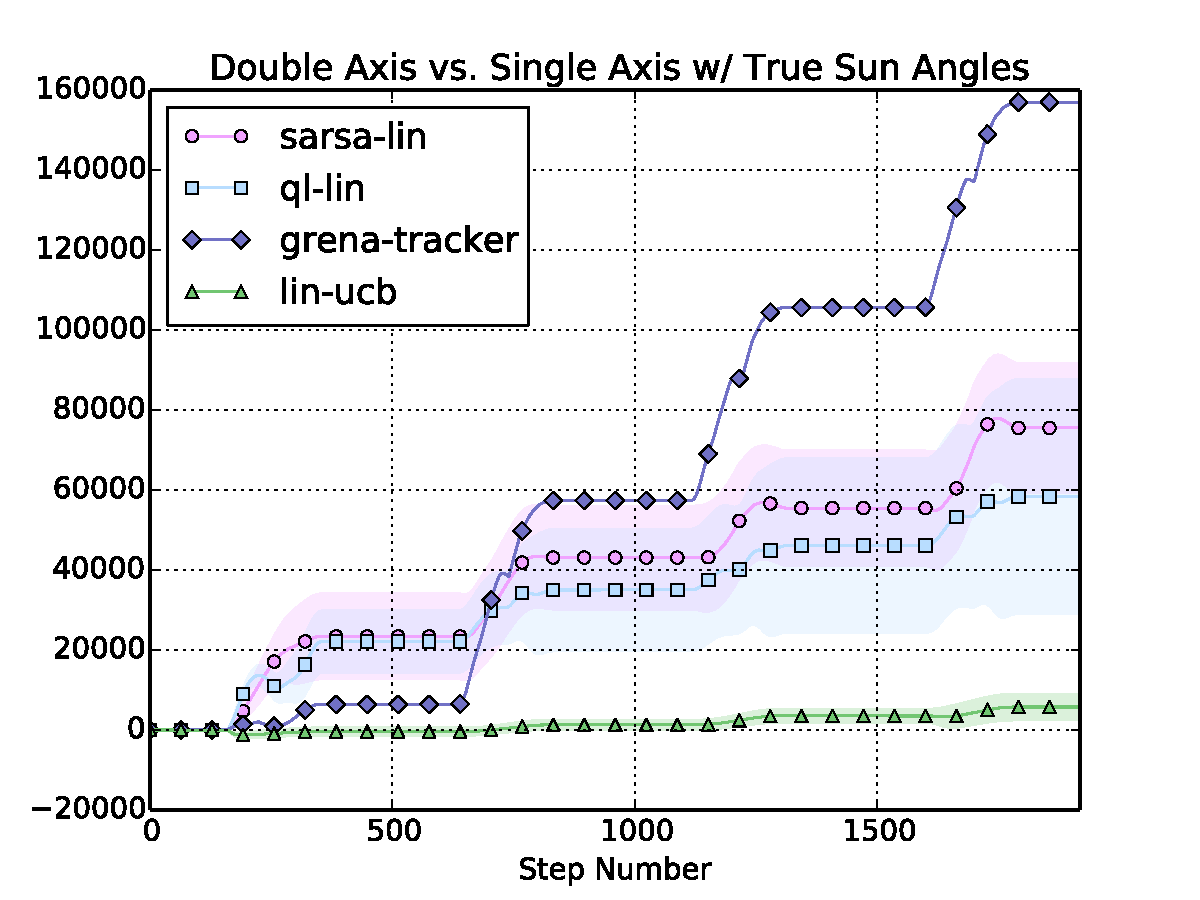
\includegraphics[scale=0.23]{figures/saxis_vs_daxis_true_cumulative}}
\subfloat[Average]{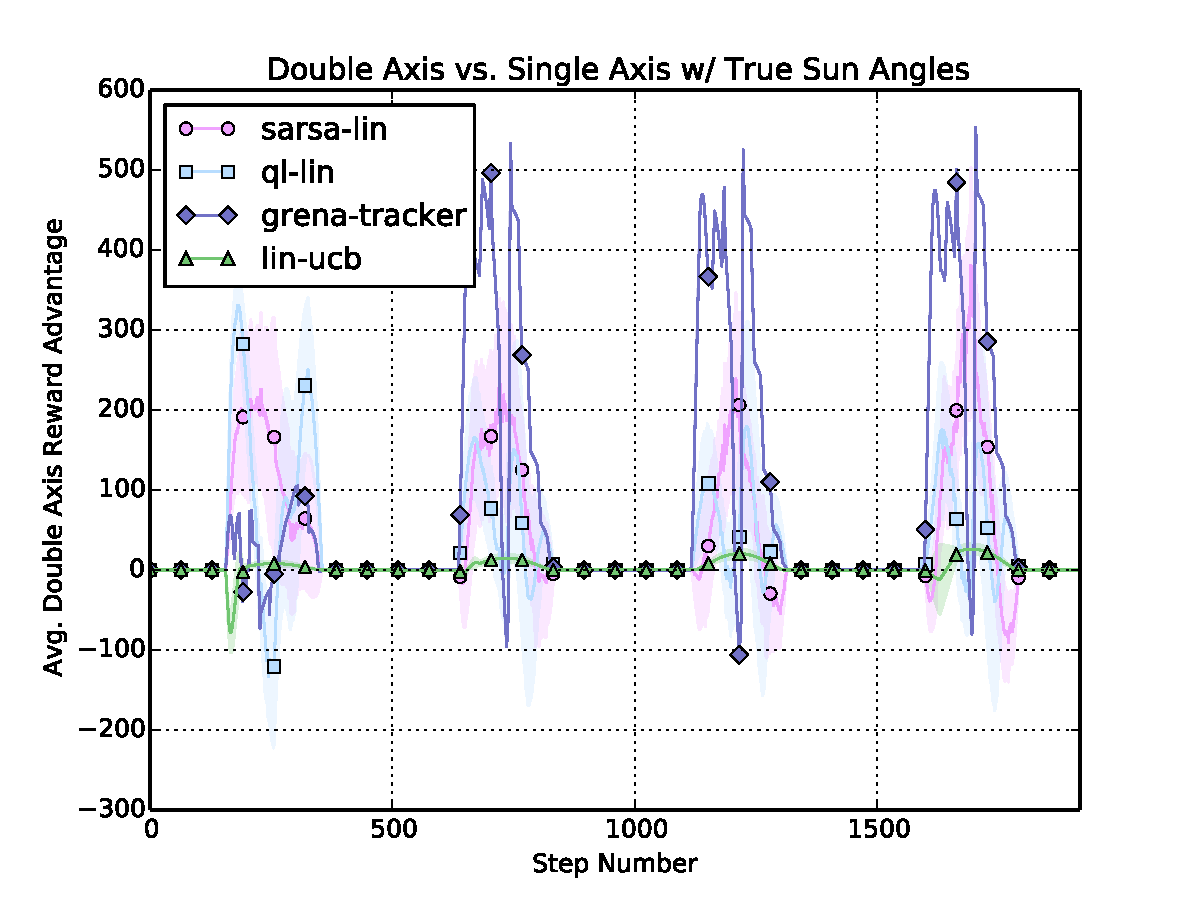
\includegraphics[scale=0.23]{figures/saxis_vs_daxis_true_avg}}
\caption{The advantage of a dual-axis over a single-axis approach with the true sun percepts, shown as cumulative difference (left) and average difference (right). Positive values indicate the dual-axis version captured more irradiance.}
\label{fig:results_axis}
\end{center}
\end{figure}


Figure~\ref{fig:results} illustrates the cumulative irradiance exposed to each panel in the Australia experiments (top) and the Iceland experiments (bottom). Notably, with the simple percept of the true sun angles, {\it all} of the learning algorithms outperform the baseline tracker and fixed panel in Australia, while in Iceland, \texttt{lin-ucb} performs worse than the \texttt{fixed} panel for the first two percepts. When just the image is provided in Australia, \texttt{lin-ucb} achieves by far the best performance; we hypothesize that this is due to LinUCB's informed approach to exploration compared to the $\varepsilon$-greedy used by \texttt{sarsa-lin} and both \texttt{ql-lin} and \texttt{ql-lin, $\gamma=0$}. Additionally, when just the sun is in the image, there is little incentive to forecast expected future reward beyond the immediate next step, which may explain the success of \texttt{lin-ucb}. This is further corroborated by the fact that \texttt{ql-lin, $\gamma=0$} does quite well in the experiment as well.

 Conversely, we see that \texttt{lin-ucb} continues to struggle in Iceland. When clouds are present, \texttt{lin-ucb} performs comparably to the other learners. The cloudy image percepts pose a challenging RL problem, but still we see that the simple approaches achieve similar performance as the \texttt{grena-tracker}, and note the substantial room for improvement from further training or more complex learners. In Iceland, the results are largely the same as Australia, though we note that the \texttt{grena-tracker} does better. In all cases, we note that there is room for improvement, suggesting that more sophisticated approaches may have more success on real panels than current techniques.

In all our simulations, the \texttt{grena-tracker} consistently outperforms the \texttt{fixed-panel} by around $25\%$, consistent with previously published results~\cite{Eke2012,mousazadeh2009review,clifford2004design}. %We take this alignment as further support of the accuracy of our simulation.

Figure~\ref{fig:results_axis} shows results for experiments comparing the {\it advantage} of the two-axis controller vs.\ a single-axis controller. In all cases except for \texttt{lin-ucb}, the presence of another axis immediately improves performance. Clearly the added problem complexity of the larger state-action space doesn't detract from the quality of the policy that the RL agents learn. We also observe that \texttt{lin-ucb} barely sees any performance gain from using the dual-axis controller.





%Figure~\ref{fig:results_rho} provides results comparing the effect of different reflective indices. Since the reflection isn't part of the observation received by any of the agents, we might not expect the 








% Results (rho tests)
%\begin{figure*}
%\begin{center}
%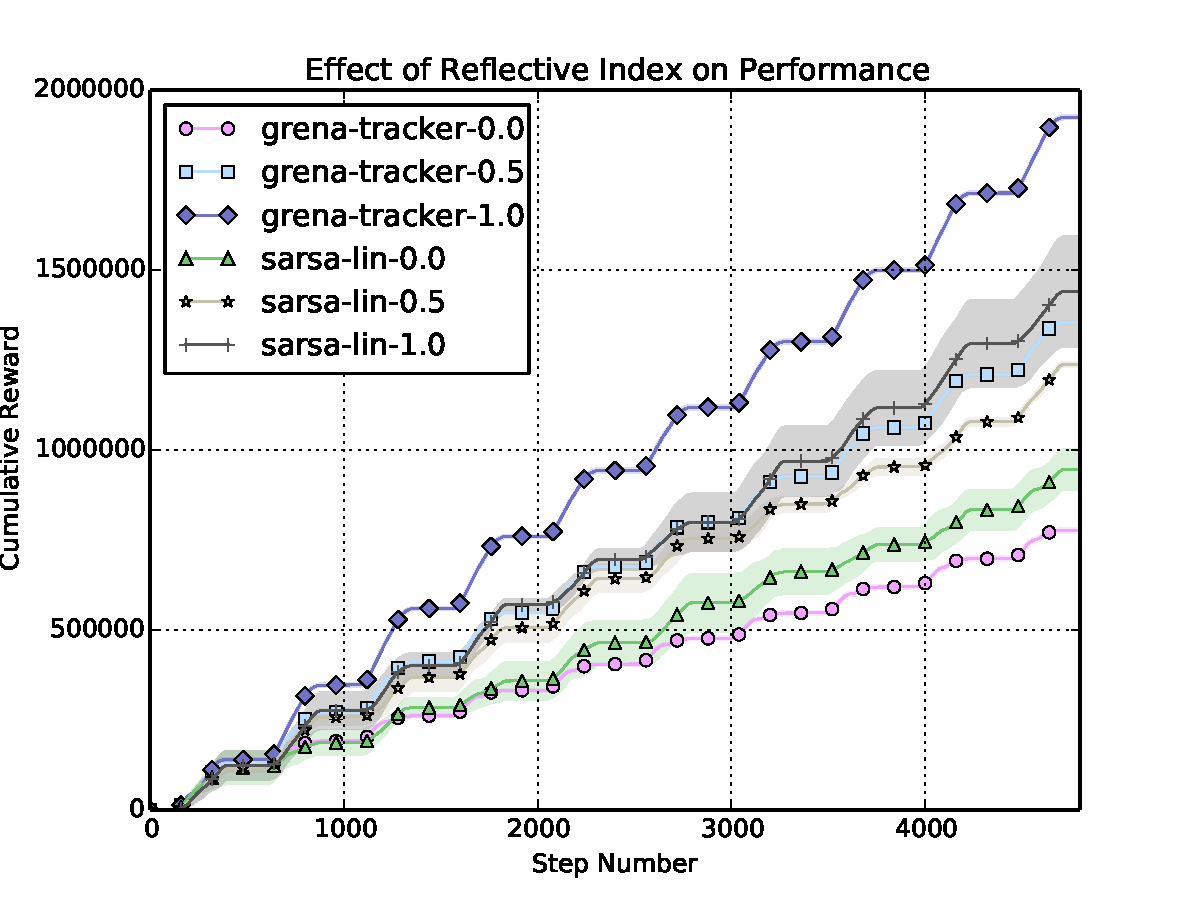
\includegraphics[scale=0.26]{figures/rho_cumulative}
%\caption{Effect of ground reflective index on energy acquired.}
%\label{fig:results_rho}
%\end{center}
%\end{figure*}



% -----------------------
% --- Conclusion ---
% -----------------------
\section{Conclusion}


We have here demonstrated the benefits of using a reinforcement-learning approach to improving the efficiency of solar panels over several established baselines. We introduced a high fidelity testbed for the problem of solar energy harvesting capable of simulating solar irradiance models anywhere on earth with a variety of generated percepts to approximate real world conditions. We take the end-to-end simulation, and the evaluation of RL on solar panel control, to be of independent interest to the broader AI and computational sustainability communities.

In the future, the natural next step is to implement a functioning RL controller on real solar panels. Additionally, there are novel algorithmic challenges posed by the solar panel setting. First, movement, observation, and computation all expend energy; incorporating these expenditures explicitly into the model poses both challenging planning and exploration questions. Second,~\citet{Hsu2015} demonstrate that simple RL approaches can optimize the problem of Maximum Power Point Tracking (MPTT) for solar panels. A system that jointly optimizes over these two criteria poses another difficult challenge.
%We are also interested in investigating transfer learning between our simulation and the real world, similar to the work of~\cite{Taylor2007}.
Lastly, we plan on applying RL to the analogous control problem presented by solar thermal energy~\cite{kalogirou2004solar}.





% ------------------------
% --- Bilbiography ---
% ------------------------
\bibliographystyle{named}
\scriptsize{\bibliography{../solar}}

\end{document}
